\subsection{Point Functions and Pointlike Functions}

\begin{remark*}[Exposition]
A metric is a two-variable distance function
\[
  d:X\times X\to\mathbb{R}_{\geq 0}.
\]
The codomain \(\mathbb{R}_{\geq 0}\) records only a nonnegative distance
value; by itself, it does not remember which point of \(X\) served as the
reference point.  Point functions adapt the metric by freezing one input.
For a fixed \(z\in X\), the function \(\delta_z:X\to\mathbb{R}_{\geq 0}\)
sends \(x\) to the distance \(d(z,x)\).  Thus a point of the metric space can
be represented by its distance profile across the whole space.
\end{remark*}

\begin{figure}[htbp]
\centering
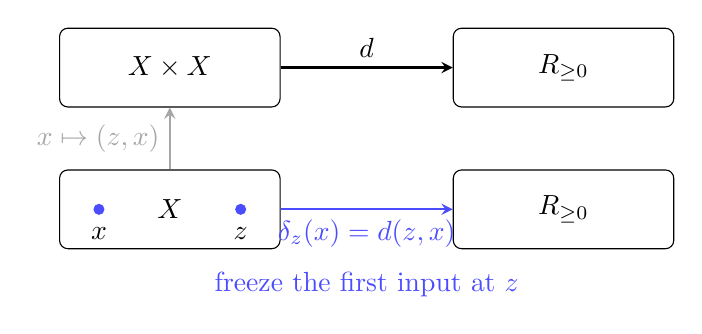
\begin{tikzpicture}[x=1cm,y=1cm,>=stealth]
  \node[draw,rounded corners=3pt,minimum width=2.8cm,minimum height=1cm]
    (product) at (0,1.6) {\(X\times X\)};
  \node[draw,rounded corners=3pt,minimum width=2.8cm,minimum height=1cm]
    (nonneg) at (5,1.6) {\(\mathbb{R}_{\geq 0}\)};
  \draw[->,thick] (product) -- node[above] {\(d\)} (nonneg);

  \node[draw,rounded corners=3pt,minimum width=2.8cm,minimum height=1cm]
    (space) at (0,-0.2) {\(X\)};
  \node[draw,rounded corners=3pt,minimum width=2.8cm,minimum height=1cm]
    (profile) at (5,-0.2) {\(\mathbb{R}_{\geq 0}\)};
  \draw[->,thick,blue!70] (space) -- node[below] {\(\delta_z(x)=d(z,x)\)} (profile);

  \draw[->,gray!70,thick] (space.north) -- node[left] {\(x\mapsto(z,x)\)} (product.south);
  \node[blue!70] at (2.5,-1.15) {freeze the first input at \(z\)};

  \fill[blue!70] (-0.9,-0.2) circle (2pt);
  \node[below=3pt] at (-0.9,-0.2) {\(x\)};
  \fill[blue!70] (0.9,-0.2) circle (2pt);
  \node[below=3pt] at (0.9,-0.2) {\(z\)};
\end{tikzpicture}

\caption{A metric \(d:X\times X\to\mathbb{R}_{\geq 0}\) becomes the point
function \(\delta_z:X\to\mathbb{R}_{\geq 0}\) when the first input is fixed at
\(z\).}
\label{fig:point-function-freezes-metric}
\end{figure}

\begin{definitionbox}{Definition --- Point Function}
\begin{definition}[Point Function]\label{def:metric-point-function}
Let \((X,d)\) be a metric space and let \(z\in X\).  The
\emph{point function at \(z\)} is the function
\[
  \delta_z:X\to\mathbb{R}_{\geq 0},
  \qquad
  \delta_z(x):=d(z,x).
\]
The set of all point functions on \(X\) is denoted by
\[
  \delta(X):=\{\,\delta_z:z\in X\,\}.
\]
\end{definition}
\end{definitionbox}

\begin{remark*}[Standard quantified statement]
\[
z\in X
\Longrightarrow
\delta_z:X\to\mathbb{R}_{\geq 0}
\quad\text{and}\quad
\forall x\in X{:}\ \delta_z(x)=d(z,x).
\]
\end{remark*}

\begin{remark*}[Interpretation]
The point function \(\delta_z\) is the distance-from-\(z\) profile.  It turns
the fixed point \(z\) into a one-variable nonnegative real-valued function on
the whole space.
\end{remark*}

\begin{remark*}[Examples]
In \(\mathbb{R}\) with the usual metric \(d(x,y)=|x-y|\), the point function
at \(z\in\mathbb{R}\) is
\[
  \delta_z(x)=d(z,x)=|x-z|.
\]
For example, the point function at \(2\) is
\[
  \delta_2(x)=|x-2|.
\]
It has value \(0\) exactly at \(x=2\), and its graph is the familiar
\(V\)-shape with vertex at \((2,0)\).  Thus the point \(2\) is encoded by the
whole distance profile \(x\mapsto |x-2|\).
\end{remark*}

\begin{dependencies}
\begin{itemize}
  \item \hyperref[def:metric-space]{Definition: Metric Space}
\end{itemize}
\end{dependencies}

\begin{theorembox}{Theorem}
\begin{theorem}[Point Functions Identify Points]
\label{thm:metric-point-functions-identify-points}
Let \((X,d)\) be a metric space.  The map
\[
  X\to\delta(X),
  \qquad
  z\mapsto\delta_z
\]
is a bijection.

\smallskip
\noindent
\hyperref[prf:metric-point-functions-identify-points]{\textit{Go to proof.}}
\end{theorem}
\end{theorembox}

\begin{remark*}[Standard quantified statement]
\[
z\mapsto\delta_z
\quad\text{is a bijection from }X\text{ onto }\delta(X).
\]
\end{remark*}

\begin{remark*}[Interpretation]
No two different points have the same distance profile.  The zero-distance
law recovers \(z\) from \(\delta_z\), because \(\delta_z(z)=0\) and no other
point has zero distance from \(z\).
\end{remark*}

\begin{dependencies}
\begin{itemize}
  \item \hyperref[def:metric-space]{Definition: Metric Space}
  \item \hyperref[def:metric-point-function]{Definition: Point Function}
\end{itemize}
\end{dependencies}

\begin{theorembox}{Theorem}
\begin{theorem}[Point Function Inequalities]
\label{thm:metric-point-function-inequalities}
Let \((X,d)\) be a nonempty metric space and let \(z\in X\).  Then, for all
\(a,b\in X\),
\[
  \delta_z(b)-\delta_z(a)\leq d(a,b)\leq \delta_z(b)+\delta_z(a),
\]
and
\[
  \delta_z(z)=0.
\]

\smallskip
\noindent
\hyperref[prf:metric-point-function-inequalities]{\textit{Go to proof.}}
\end{theorem}
\end{theorembox}

\begin{remark*}[Standard quantified statement]
\[
\forall a,b\in X{:}\quad
\delta_z(b)-\delta_z(a)\leq d(a,b)\leq \delta_z(b)+\delta_z(a),
\qquad
\delta_z(z)=0.
\]
\end{remark*}

\begin{remark*}[Interpretation]
Point functions mimic the metric because they are built from the metric.  The
right-hand inequality is the triangle inequality through \(z\), while the
left-hand inequality is the reverse triangle estimate.
\end{remark*}

\begin{dependencies}
\begin{itemize}
  \item \hyperref[def:metric-space]{Definition: Metric Space}
  \item \hyperref[def:metric-point-function]{Definition: Point Function}
\end{itemize}
\end{dependencies}

\begin{definitionbox}{Definition --- Pointlike Function}
\begin{definition}[Pointlike Function]\label{def:metric-pointlike-function}
Let \((X,d)\) be a nonempty metric space.  A function
\[
  u:X\to\mathbb{R}_{\geq 0}
\]
is \emph{pointlike} on \(X\) if, for all \(a,b\in X\),
\[
  u(a)-u(b)\leq d(a,b)\leq u(a)+u(b).
\]
\end{definition}
\end{definitionbox}

\begin{remark*}[Standard quantified statement]
\[
u\text{ is pointlike}
\quad\Longleftrightarrow\quad
u:X\to\mathbb{R}_{\geq 0}
\;\land\;
\forall a,b\in X{:}\ u(a)-u(b)\leq d(a,b)\leq u(a)+u(b).
\]
\end{remark*}

\begin{remark*}[Interpretation]
A pointlike function satisfies the inequalities that every point function
satisfies.  It behaves like a distance-from-something profile, even before a
point realizing that profile has been identified.
\end{remark*}

\begin{dependencies}
\begin{itemize}
  \item \hyperref[def:metric-space]{Definition: Metric Space}
  \item \hyperref[thm:metric-point-function-inequalities]{Theorem: Point Function Inequalities}
\end{itemize}
\end{dependencies}

\begin{theorembox}{Theorem}
\begin{theorem}[Pointlike Functions with a Zero Are Point Functions]
\label{thm:metric-pointlike-zero-point-function}
Let \((X,d)\) be a metric space and let \(u:X\to\mathbb{R}_{\geq 0}\).  Then
\(u\in\delta(X)\) if and only if \(u\) is pointlike on \(X\) and
\[
  0\in u(X).
\]
In that case, there is a unique \(w\in X\) such that \(u(w)=0\), and
\[
  u=\delta_w.
\]

\smallskip
\noindent
\hyperref[prf:metric-pointlike-zero-point-function]{\textit{Go to proof.}}
\end{theorem}
\end{theorembox}

\begin{remark*}[Standard quantified statement]
\[
u\in\delta(X)
\quad\Longleftrightarrow\quad
u\text{ is pointlike on }X
\;\land\;
0\in u(X).
\]
\end{remark*}

\begin{remark*}[Interpretation]
The zero value anchors a pointlike function to an actual point of \(X\).  Once
\(u(w)=0\), the pointlike inequalities force \(u(a)=d(w,a)\) for every
\(a\in X\), so \(u\) is exactly the point function \(\delta_w\).
\end{remark*}

\begin{dependencies}
\begin{itemize}
  \item \hyperref[def:metric-point-function]{Definition: Point Function}
  \item \hyperref[def:metric-pointlike-function]{Definition: Pointlike Function}
\end{itemize}
\end{dependencies}
